\documentclass[10pt,fleqn]{article}
\newcommand{\name}[1]{\def\psettitlename{#1}}
\newcommand{\course}[1]{\def\psettitlecourse{#1}}
\newcommand{\rsection}[1]{\def\psettitlersection{#1}}
\newcommand{\psetnum}[1]{\def\psettitlepsetnum{#1}}
% \usepackage[journal=rsc]{chemstyle}
% \usepackage{mhchem}
\usepackage{amsmath}
\usepackage{amssymb}
\usepackage{amsfonts}
\usepackage{esint}
\usepackage{bbm}
\usepackage{amscd}
\usepackage{picinpar}
\usepackage[pdftex]{graphicx}
\usepackage{indentfirst}
\usepackage{wrapfig}
\usepackage{units}
\usepackage{textcomp}
\usepackage[utf8x]{inputenc}
\usepackage{feyn}
\usepackage{feynmp}
\DeclareGraphicsRule{*}{mps}{*}{}
\newcommand{\ud}{\mathrm{d}}
\newcommand{\ue}{\mathrm{e}}
\newcommand{\ui}{\mathrm{i}}
\newcommand{\res}{\mathrm{Res}}
\newcommand{\Tr}{\mathrm{Tr}}
\newcommand{\dsum}{\displaystyle\sum}
\newcommand{\dprod}{\displaystyle\prod}
\newcommand{\dlim}{\displaystyle\lim}
\newcommand{\dint}{\displaystyle\int}
\newcommand{\fsno}[1]{{\!\not\!{#1}}}
\newcommand{\eqar}[1]
{
  \begin{align*}
    #1
  \end{align*}
}
\newcommand{\texp}[2]{\ensuremath{{#1}\times10^{#2}}}
\newcommand{\dexp}[2]{\ensuremath{{#1}\cdot10^{#2}}}
\newcommand{\eval}[2]{{\left.{#1}\right|_{#2}}}
\newcommand{\paren}[1]{{\left({#1}\right)}}
\newcommand{\lparen}[1]{{\left({#1}\right.}}
\newcommand{\rparen}[1]{{\left.{#1}\right)}}
\newcommand{\abs}[1]{{\left|{#1}\right|}}
\newcommand{\sqr}[1]{{\left[{#1}\right]}}
\newcommand{\crly}[1]{{\left\{{#1}\right\}}}
\newcommand{\angl}[1]{{\left\langle{#1}\right\rangle}}
\newcommand{\tpdiff}[4][{}]{{\paren{\frac{\partial^{#1} {#2}}{\partial {#3}{}^{#1}}}_{#4}}}
\newcommand{\tpsdiff}[4][{}]{{\paren{\frac{\partial^{#1}}{\partial {#3}{}^{#1}}{#2}}_{#4}}}
\newcommand{\pdiff}[3][{}]{{\frac{\partial^{#1} {#2}}{\partial {#3}{}^{#1}}}}
\newcommand{\diff}[3][{}]{{\frac{\ud^{#1} {#2}}{\ud {#3}{}^{#1}}}}
\newcommand{\psdiff}[3][{}]{{\frac{\partial^{#1}}{\partial {#3}{}^{#1}} {#2}}}
\newcommand{\sdiff}[3][{}]{{\frac{\ud^{#1}}{\ud {#3}{}^{#1}} {#2}}}
\newcommand{\tpddiff}[4][{}]{{\left(\dfrac{\partial^{#1} {#2}}{\partial {#3}{}^{#1}}\right)_{#4}}}
\newcommand{\tpsddiff}[4][{}]{{\paren{\dfrac{\partial^{#1}}{\partial {#3}{}^{#1}}{#2}}_{#4}}}
\newcommand{\pddiff}[3][{}]{{\dfrac{\partial^{#1} {#2}}{\partial {#3}{}^{#1}}}}
\newcommand{\ddiff}[3][{}]{{\dfrac{\ud^{#1} {#2}}{\ud {#3}{}^{#1}}}}
\newcommand{\psddiff}[3][{}]{{\frac{\partial^{#1}}{\partial{}^{#1} {#3}} {#2}}}
\newcommand{\sddiff}[3][{}]{{\frac{\ud^{#1}}{\ud {#3}{}^{#1}} {#2}}}
\usepackage{fancyhdr}
\usepackage{multirow}
\usepackage{fontenc}
% \usepackage{tipa}
\usepackage{ulem}
\usepackage{color}
\usepackage{cancel}
\newcommand{\hcancel}[2][black]{\setbox0=\hbox{#2}%
  \rlap{\raisebox{.45\ht0}{\textcolor{#1}{\rule{\wd0}{1pt}}}}#2}
\pagestyle{fancy}
\setlength{\headheight}{67pt}
\fancyhead{}
\fancyfoot{}
\fancyfoot[C]{\thepage}
\fancyhead[R]
{
  \psettitlename \\
  \psettitlecourse{} Problem Set \psettitlepsetnum \\
  \ifx\psettitlersection\empty
  \else
  Recitation Section \psettitlersection
  \fi
}
\renewcommand{\footruleskip}{0pt}
\renewcommand{\headrulewidth}{0.4pt}
\renewcommand{\footrulewidth}{0pt}
\addtolength{\hoffset}{-1.3cm}
\addtolength{\voffset}{-2cm}
\addtolength{\textwidth}{3cm}
\addtolength{\textheight}{2.5cm}
\renewcommand{\footskip}{10pt}
\setlength{\headwidth}{\textwidth}
\setlength{\headsep}{20pt}
\setlength{\marginparwidth}{0pt}
\parindent=0pt
\psetnum{5}
\course{Physics 251b}
\rsection{1}
\name{Yichao Yu}
\renewcommand{\thesection}{\arabic{section}.}
\renewcommand{\thesubsection}{(\alph{subsection})}
\renewcommand{\thesubsubsection}{\roman{subsubsection}.}

\begin{document}
\section{Gauge invariance and the Lorentz force}
\subsection{}
Schroedinger equation
\eqar{
  \ui\hbar\pdiff{\psi}{t}=&-\frac{\hbar^2}{2m}\paren{\nabla-\frac{\ui q}{\hbar c}\vec A}^2\psi+q\phi\psi
  \intertext{Complex conjugate}
  -\ui\hbar\pdiff{\psi^*}{t}=&-\frac{\hbar^2}{2m}\paren{\nabla+\frac{\ui q}{\hbar c}\vec A}^2\psi^*+q\phi\psi^*\\
  \ui\hbar\psi^*\pdiff{\psi}{t}=&-\psi^*\frac{\hbar^2}{2m}\paren{\nabla-\frac{\ui q}{\hbar c}\vec A}^2\psi+q\phi\psi^*\psi\\
  -\ui\hbar\psi\pdiff{\psi^*}{t}=&-\frac{\hbar^2}{2m}\psi\paren{\nabla+\frac{\ui q}{\hbar c}\vec A}^2\psi^*+q\phi\psi^*\psi\\
  \ui\hbar\pdiff{\psi^*\psi}{t}=&-\psi^*\frac{\hbar^2}{2m}\paren{\nabla-\frac{\ui q}{\hbar c}\vec A}^2\psi+\frac{\hbar^2}{2m}\psi\paren{\nabla+\frac{\ui q}{\hbar c}\vec A}^2\psi^*\\
  =&-\frac{\hbar^2}{2m}\paren{\nabla\paren{\psi^*\paren{\nabla-\frac{\ui q}{\hbar c}\vec A}\psi}-\abs{\paren{\nabla-\frac{\ui q}{\hbar c}\vec A}\psi}^2}\\
  &+\frac{\hbar^2}{2m}\paren{\nabla\paren{\psi\paren{\nabla+\frac{\ui q}{\hbar c}\vec A}\psi^*}-\abs{\paren{\nabla-\frac{\ui q}{\hbar c}\vec A}\psi}^2}\\
  =&\frac{\hbar^2}{2m}\nabla\paren{\psi\paren{\nabla+\frac{\ui q}{\hbar c}\vec A}\psi^*-\psi^*\paren{\nabla-\frac{\ui q}{\hbar c}\vec A}\psi}\\
  \pdiff{\rho}{t}=&\frac{\hbar}{2m\ui}\nabla\paren{\psi\paren{\nabla+\frac{\ui q}{\hbar c}\vec A}\psi^*-\psi^*\paren{\nabla-\frac{\ui q}{\hbar c}\vec A}\psi}\\
  =&-\nabla\cdot\vec j\\
  0=&\pdiff{\rho}{t}+\nabla\cdot\vec j
}
\subsection{}
Under time reversal transformation
\eqar{
  &-\ui\hbar\pdiff{\psi^*}{t}+\frac{\hbar^2}{2m}\paren{\nabla-\frac{\ui q}{\hbar c}\vec A}^2\psi^*-q\phi\psi^*\\
  =&\frac{\hbar^2}{2m}\paren{\paren{\nabla-\frac{\ui q}{\hbar c}\vec A}^2-\paren{\nabla+\frac{\ui q}{\hbar c}\vec A}^2}\psi^*\\
  \neq&0
}
\subsection{}
Derivatives,
\eqar{
  \pdiff{L}{\dot r_i}=&m\dot r_i+\frac{q}{c}A_i\\
  \pdiff{L}{r_i}=&-q\partial_i\phi+\frac{q}{c}\dot r_j\partial_iA_j
  \intertext{Euler-Lagrange equation}
  0=&m\ddot r_i+\frac{q}{c}\diff{A_i}{t}+q\partial_i\phi-\frac{q}{c}\dot r_j\partial_iA_j\\
  m\ddot r_i=&-\frac{q}{c}\diff{A_i}{t}-q\partial_i\phi+\frac{q}{c}\dot r_j\partial_iA_j\\
  =&-q\partial_i\phi-\frac{q}{c}\partial_tA_i-\frac{q}{c}\dot r_j\partial_jA_i+\frac{q}{c}\dot r_j\partial_iA_j\\
  =&qE_i+\frac{q}{c}\paren{\delta_{ln}\delta_{im}-\delta_{lm}\delta_{in}}\dot r_l\partial_mA_n\\
  =&qE_i+\frac{q}{c}\varepsilon_{ilj}\dot r_l\varepsilon_{jmn}\partial_mA_n\\
  =&qE_i+\frac{q}{c}\varepsilon_{ilj}\dot r_lB_j\\
  =&qE_i+\frac{q}{c}\paren{\vec v\times\vec B}_i
}
\section{}
\subsection{}
For each step
\eqar{
  K(x_{j+1},x_j;\varepsilon)=&\sqrt{\frac{m}{2\pi\ui\hbar\varepsilon}}\exp\paren{\frac{\ui}{\hbar}\paren{a_1\paren{x^2_{j+1}+x_j^2}-2b_1x_{j+1}x_j}}
}
where $a_1\equiv\dfrac{m}{2\varepsilon}\paren{1-2\paren{\dfrac{\omega\varepsilon}{2}}^2}$, $b_1\equiv\dfrac{m}{2\varepsilon}$. Assume,
\eqar{
  &\paren{\frac{m}{2\pi\ui\hbar\varepsilon}}^{n/2}\prod_{j=1}^n\int\ud x_{j-1}\exp\paren{\frac{\ui}{\hbar}\sum_{j=1}^n\paren{a_1\paren{x^2_{j-1}+x_j^2}-2b_1x_{j-1}x_j}}\\
  =&A_n\exp\paren{\frac{\ui}{\hbar}\paren{a_n\paren{x^2_{n}+x_{0}^2}-2b_nx_{n}x_{0}}}
  \intertext{and $a_n^2-b_n^2=a_1^2-b_1^2$}
  &A_{n+1}\exp\paren{\frac{\ui}{\hbar}\paren{a_{n+1}\paren{x^2_{0}+x_{n+1}^2}-2b_{n+1}x_{0}x_{n+1}}}\\
  =&A_n\paren{\frac{m}{2\pi\ui\hbar\varepsilon}}^{1/2}\int\ud x_n\exp\paren{\frac{\ui}{\hbar}\paren{a_1\paren{x^2_{n+1}+x_n^2}-2b_1x_{n+1}x_n+a_n\paren{x^2_{n}+x_{0}^2}-2b_nx_{n}x_{0}}}\\
  =&A_n\paren{\frac{m}{2\pi\ui\hbar\varepsilon}}^{1/2}
  \int\ud x_n\exp\paren{\frac{\ui}{\hbar}\paren{\paren{a_1+a_n}x_n^2-2\paren{b_1x_{n+1}+b_nx_0}x_n+a_1x^2_{n+1}+a_nx_{0}^2}}\\
  =&A_n\paren{\frac{m}{2\pi\ui\hbar\varepsilon}}^{1/2}
  \sqrt{\frac{\ui\pi\hbar}{a_1+a_n}}
  \exp\paren{\frac{\ui}{\hbar}\paren{-\frac{\paren{b_1x_{n+1}+b_nx_0}^2}{a_1+a_n} + a_1x^2_{n+1}+a_nx_{0}^2}}\\
  =&A_n\paren{\frac{m}{2\pi\ui\hbar\varepsilon}}^{1/2}
  \sqrt{\frac{\ui\pi\hbar}{a_1+a_n}}
  \exp\paren{\frac{\ui}{\hbar}\paren{
      \paren{a_1-\frac{b_1^2}{a_1+a_n}}\paren{x_{n+1}^2+x_0^2}
      -2\frac{b_1b_n}{a_1+a_n}x_{n+1}x_0}
  }
}
So $a_{n+1}=a_1-\dfrac{b_1^2}{a_1+a_n}$, $b_{n+1}=\dfrac{b_1b_n}{a_1+a_n}$,
which also satisfy $a_{n+1}^2-b_{n+1}^2=a_1^2-b_1^2$.
Let $\dfrac{\omega\varepsilon}{2}=\sin\dfrac{\tilde\omega\varepsilon}{2}$
\eqar{
  a_1=&b_1\cos\tilde\omega\varepsilon\\
  a_n=&\sqrt{b_n^2-b_1^2\sin^2\tilde\omega\varepsilon}\\
  \frac1{b_{n+1}}=&\dfrac{\cos\tilde\omega\varepsilon+\sqrt{\dfrac{b_n^2}{b_1^2}-\sin^2\tilde\omega\varepsilon}}{b_n}\\
  \frac1{b_n}=&\frac{\sin n\tilde\omega\varepsilon}{b_1\sin\tilde\omega\varepsilon}\\
  a_n=&\frac{m\sin\tilde\omega\varepsilon}{2\varepsilon}\frac{\cos n\tilde\omega\varepsilon}{\sin n\tilde\omega\varepsilon}
}
In the small $\varepsilon$ limit and when $n=N$
\eqar{
  \frac1{b}=&\frac{2\sin\omega t}{m\omega}\\
  a=&\frac{m\omega}{2\sin\omega t}\cos\omega t
}
Therefore the full propagator takes the form
\eqar{
  A\exp\paren{\frac{\ui m\omega}{2\hbar\sin\omega t}\paren{\cos\omega t\paren{x^2+x'^2}-2xx'}}
}
\subsection{}
\eqar{
  K=&\sqrt{\frac{m\omega}{2\pi\ui\hbar\sin\omega t}}\\
  =&\sqrt{\frac{m\omega}{\pi\hbar}}\paren{2\ui\sin\omega t}^{-1/2}\\
  =&\sqrt{\frac{m\omega}{\pi\hbar}}\paren{\ue^{\ui\omega t}-\ue^{-\ui\omega t}}^{-1/2}\\
  =&\sqrt{\frac{m\omega}{\pi\hbar}}\ue^{-\ui\omega t/2}\paren{1-\ue^{-2\ui\omega t}}^{-1/2}\\
  =&\sqrt{\frac{m\omega}{\pi\hbar}}\ue^{-\ui\omega t/2}\sum_{i=0}^\infty a_n\ue^{-2\ui\omega t}
}
where $a_n$ is the expansion coefficient of $(1-x)^{1/2}$.
The states in between are missing due to the zero in the wavefunction.
\subsection{}
\eqar{
  K=&\sqrt{\frac{m\omega}{2\pi\ui\hbar\sin\omega t}}\exp\paren{\frac{\ui m\omega x^2}{\hbar\sin\omega t}\paren{\cos\omega t-1}}
  \intertext{Trace}
  \int K\ud x=&\sqrt{\frac{m\omega}{2\pi\ui\hbar\sin\omega t}}\exp\paren{\frac{\ui m\omega x^2}{\hbar\sin\omega t}\paren{\cos\omega t-1}}\\
  =&\sqrt{\frac{m\omega}{2\pi\ui\hbar\sin\omega t}\frac{\ui\pi\hbar\sin\omega t}{m\omega\paren{\cos\omega t - 1}}}\\
  =&\sqrt{\frac{1}{\paren{\cos\omega t - 1}}}\\
  =&\frac{1}{2\ui\sin\paren{\omega t/2}}\\
  =&\paren{\ue^{\ui\omega t/2}-\ue^{-\ui\omega t/2}}^{-1}\\
  =&\ue^{-\ui\omega t/2}\paren{1-\ue^{-\ui\omega t}}^{-1}\\
  =&\sum_{n=0}^\infty\exp\paren{-\ui\omega t\paren{n+\frac12}}
}
\section{}
\subsection{}
Function to minimize
\eqar{
  E=&\int\ud^3r\varphi^*H\varphi-\varepsilon\paren{\int\ud^3r\varphi^*\varphi-1}\\
  =&\int\ud^3r\paren{\alpha\psi_A+\beta\psi_B}\paren{-\frac{\hbar^2}{2m}\nabla^2-\frac{e^2}{r_{1A}}-\frac{e^2}{r_{1B}}+\frac{e^2}{R}}\paren{\alpha\psi_A+\beta\psi_B}\\
  &-\varepsilon\paren{\int\ud^3r\paren{\alpha\psi_A+\beta\psi_B}^2-1}
  \intertext{Expanding derivative around the center of the wavefunctions}
  E=&\alpha\int\ud^3r\paren{\alpha\psi_A+\beta\psi_B}\paren{E_{1s}-\frac{e^2}{r_{1B}}+\frac{e^2}{R}}\psi_A\\
  &+\beta\int\ud^3r\paren{\alpha\psi_A+\beta\psi_B}\paren{E_{1s}-\frac{e^2}{r_{1A}}+\frac{e^2}{R}}\psi_B\\
  &-\varepsilon\paren{\int\ud^3r\paren{\alpha\psi_A+\beta\psi_B}^2-1}\\
  =&\alpha^2\paren{E_{1s}-e^2\int\ud^3r\frac{\psi_A^2}{r_{1B}}+\frac{e^2}{R}}+\alpha\beta\paren{E_{1s}S+\frac{e^2S}{R}-e^2\int\ud^3r\frac{\psi_A\psi_B}{r_{1B}}}\\
  &+\beta^2\paren{E_{1s}-e^2\int\ud^3r\frac{\psi_B^2}{r_{1A}}+\frac{e^2}{R}}+\alpha\beta\paren{E_{1s}S+\frac{e^2S}{R}-e^2\int\ud^3r\frac{\psi_A\psi_B}{r_{1A}}}\\
  &-\varepsilon\paren{\alpha^2+2\alpha\beta S+\beta^2-1}
  \intertext{Let $U_1\equiv\dint\ud^3r\dfrac{\psi_A^2}{r_{1B}}=\dint\ud^3r\dfrac{\psi_B^2}{r_{1A}}$, $U_2\equiv\dint\ud^3r\dfrac{\psi_A\psi_B}{r_{1A}}=\dint\ud^3r\dfrac{\psi_A\psi_B}{r_{1B}}$}
  E=&\paren{\alpha^2+\beta^2}\paren{E_{1s}-e^2U_1+\frac{e^2}{R}-\varepsilon}+2\alpha\beta\paren{E_{1s}S+\frac{e^2S}{R}-e^2U_2-\varepsilon S}-\varepsilon\\
  =&-\paren{\alpha^2+\beta^2}\paren{e^2U_1+\zeta}-2\alpha\beta\paren{e^2U_2+\zeta S}-\varepsilon
  \intertext{To minimize $E$}
  0=&\alpha^2+2\alpha\beta S+\beta^2-1\\
  0=&\alpha\paren{e^2U_1+\zeta}+\beta\paren{e^2U_2+\zeta S}\\
  0=&\beta\paren{e^2U_1+\zeta}+\alpha\paren{e^2U_2+\zeta S}
  \intertext{Therefore,}
  V_{AA}=&V_{BB}=e^2U_1\\
  V_{AB}=&V_{BA}=e^2U_2
}
\subsection{}
From normalization,
\eqar{
  \alpha=&\frac{1}{\sqrt{2\paren{1+S}}}
  \intertext{Energy}
  \varepsilon=&2\alpha^2\paren{E_{1s}-e^2U_1+\frac{e^2}{R}}+2\alpha^2\paren{E_{1s}S+\frac{e^2S}{R}-e^2U_2}\\
  =&\frac{1}{1+S}\paren{\paren{E_{1s}+\frac{e^2}{R}}\paren{1+S}-e^2U_1-e^2U_2}\\
  =&E_{1s}+\frac{e^2}{R}-\frac{e^2}{1+\paren{1+\rho+\rho^2/3}\ue^{-\rho}}\paren{\frac{1}{R}\paren{1-\paren{1+\rho}\ue^{-2\rho}}+\frac{1}{a_0}\paren{1+\rho}\ue^{-\rho}}\\
  f=&\frac{1-2\rho^2/3+\paren{1+\rho}\ue^{-\rho}}{1+\paren{1+\rho+\rho^2/3}\ue^{-\rho}}\ue^{-\rho}
}
\subsection{}
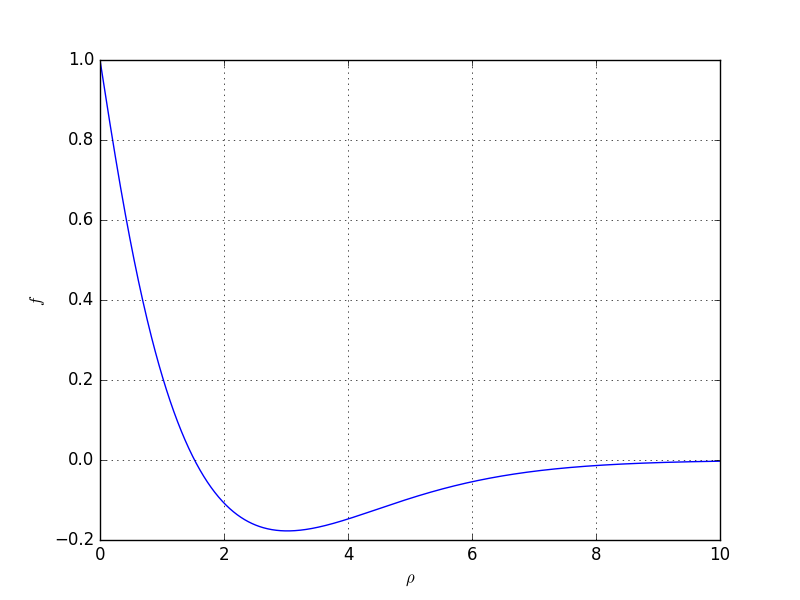
\includegraphics[width=10cm]{3c.png}\\
The potential is minimized when $\rho=3$
\section{}
\subsection{}
Eigenvalue equation
\eqar{
  (\varepsilon-\lambda)^2=&t^2\\
  \varepsilon-\lambda=&\pm t\\
  \lambda=&\varepsilon\pm t
}
Eigenvectors $r_1|R\rangle+r_2|R'\rangle$
\eqar{
  0=&\paren{\varepsilon-\lambda}r_1-tr_2\\
  r_2=&\mp r_1
  \intertext{Normalized eigenvectors}
  |\psi\rangle=&\frac1{\sqrt2}\paren{|R\rangle\mp|R'\rangle}
}
\subsection{}
\eqar{
  |\Phi_H\rangle=&\frac12\paren{|R_1\rangle+|R_1'\rangle}\paren{|R_2\rangle+|R_2'\rangle}\\
  =&\frac12\paren{|RR\rangle+|RR'\rangle+|R'R\rangle+|R'R'\rangle}\\
  =&\frac{1}{\sqrt2}|\Phi_0\rangle+\frac{1}{2}\paren{|\Phi_1\rangle+|\Phi_2\rangle}\\
  E_H=&2\paren{\varepsilon-t}+U
}
Matrix elements
\eqar{
  h_1=&\begin{pmatrix}
    \langle \Phi_0|h_1|\Phi_0\rangle&\langle \Phi_0|h_1|\Phi_1\rangle&\langle \Phi_0|h_1|\Phi_2\rangle\\
    \langle \Phi_1|h_1|\Phi_0\rangle&\langle \Phi_1|h_1|\Phi_1\rangle&\langle \Phi_1|h_1|\Phi_2\rangle\\
    \langle \Phi_2|h_1|\Phi_0\rangle&\langle \Phi_2|h_1|\Phi_1\rangle&\langle \Phi_2|h_1|\Phi_2\rangle
  \end{pmatrix}\\
  =&\begin{pmatrix}
    \dfrac{1}{2}\paren{\langle R|h_1|R\rangle+\langle R'|h_1|R'\rangle}&\dfrac{1}{\sqrt2}\langle R'|h_1|R\rangle&\dfrac{1}{\sqrt2}\langle R|h_1|R'\rangle\\
    \dfrac{1}{\sqrt2}\langle R|h_1|R'\rangle&\langle R|h_1|R\rangle&0\\
    \dfrac{1}{\sqrt2}\langle R'|h_1|R\rangle&0&\langle R'|h_1|R'\rangle
  \end{pmatrix}\\
  =&\begin{pmatrix}
    \varepsilon&\dfrac{t}{\sqrt2}&\dfrac{t}{\sqrt2}\\
    \dfrac{t}{\sqrt2}&\varepsilon&0\\
    \dfrac{t}{\sqrt2}&0&\varepsilon
  \end{pmatrix}
  \intertext{Similarly}
  h_2=&\begin{pmatrix}
    \varepsilon&\dfrac{t}{\sqrt2}&\dfrac{t}{\sqrt2}\\
    \dfrac{t}{\sqrt2}&\varepsilon&0\\
    \dfrac{t}{\sqrt2}&0&\varepsilon
  \end{pmatrix}\\
  V_{12}=&\begin{pmatrix}
    0&0&0\\
    0&U&0\\
    0&0&U
  \end{pmatrix}\\
  H=&\begin{pmatrix}
    2\varepsilon&\sqrt2t&\sqrt2t\\
    \sqrt2t&2\varepsilon+U&0\\
    \sqrt2t&0&2\varepsilon+U
  \end{pmatrix}
}
$\alpha=\sqrt2$
\subsection{}
\eqar{
  0=&\paren{2\varepsilon-\lambda}\paren{2\varepsilon+U-\lambda}^2-4t^2\paren{2\varepsilon+U-\lambda}\\
  \lambda_1=&2\varepsilon+U\\
  0=&\paren{2\varepsilon-\lambda}\paren{2\varepsilon+U-\lambda}-4t^2\\
  0=&\paren{2\varepsilon-\lambda}^2+U\paren{2\varepsilon-\lambda}-4t^2\\
  \lambda_{2,3}=&2\varepsilon+\frac{U\pm\sqrt{U^2+16t^2}}{2}
}
Therefore $E_{exact}=2\varepsilon+\dfrac{U-\sqrt{U^2+16t^2}}{2}$\\
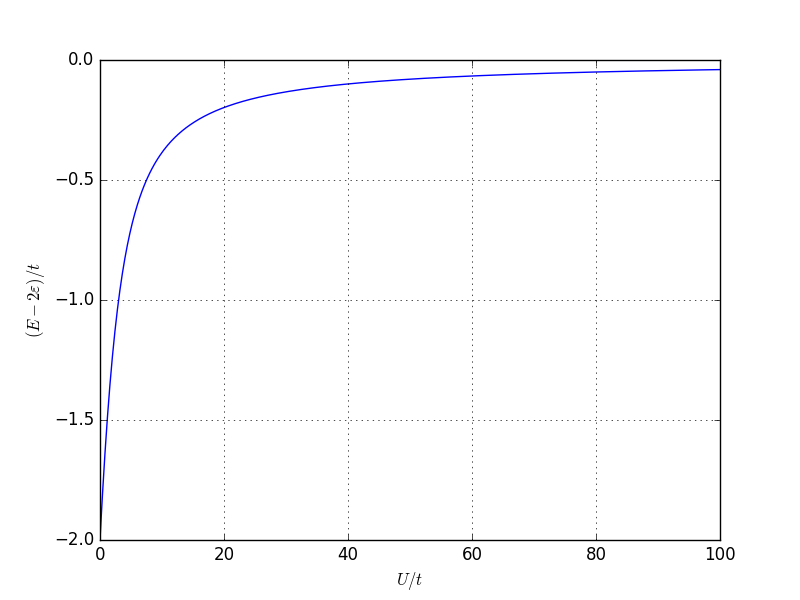
\includegraphics[width=10cm]{4c.png}\\
For small $u$ this fallback to the non-interacting case, for large $U$, this fallback to separate atom case.
\subsection{}
The eigenstate corresponds to $\lambda_1$ is $|\Phi_1\rangle-|\Phi_2\rangle$
so other eigenstates has to take the form $\dfrac{1}{\sqrt2}|\Phi_0\rangle+\frac{f(u)}{2}\paren{|\Phi_1\rangle+|\Phi_2\rangle}$ in order to be orthogonal to it.
Substitute to $H$
\eqar{
  0=&\sqrt2t\frac{1}{\sqrt{2}}+\dfrac{U+\sqrt{U^2+16t^2}}{2}\frac{f}{2}\\
  f=&-\frac{4t}{U+\sqrt{U^2+16t^2}}\\
  =&\frac{u-\sqrt{u^2+16}}{4}
}
The probability of finding two electron on the same proton is $\dfrac{f^2}{1+f^2}$\\
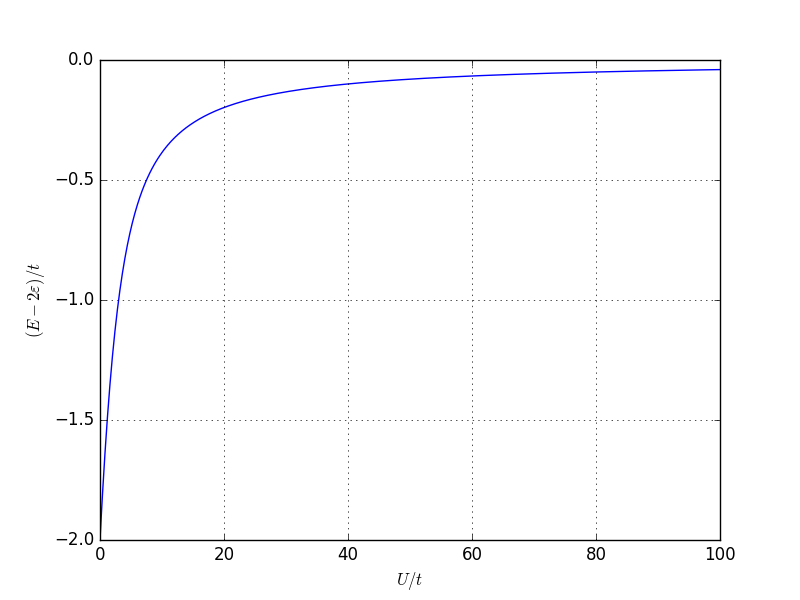
\includegraphics[width=10cm]{4c.png}\\
For small $u$ this fallback to the non-interacting case, for large $U$, the atom will stay on different protons due to repulsion.
\end{document}
